\subsection{Can}

\begin{frame}
<<<<<<< HEAD
\frametitle{Gimbal}

  %\begin{figure}
  %\includegraphics[scale=0.6, trim={5cm 8.5cm 5.5cm 8.5cm},clip]{pic/03_content/Serial_output.pdf}
  %\end{figure}
=======
\frametitle{Self build kit}

  \begin{itemize}
    \item No special knowledge required    
	\item Very sturdy
	\item Many tools
	\item Payload    
	\item Price-Performance ratio
  \end{itemize}
>>>>>>> origin/master
  
\end{frame}



<<<<<<< HEAD

\begin{frame}
\frametitle{GPS navigation}

  \begin{itemize}
    \item Waypoints    
=======
\begin{frame}
\frametitle{Payload}

  \begin{figure}
  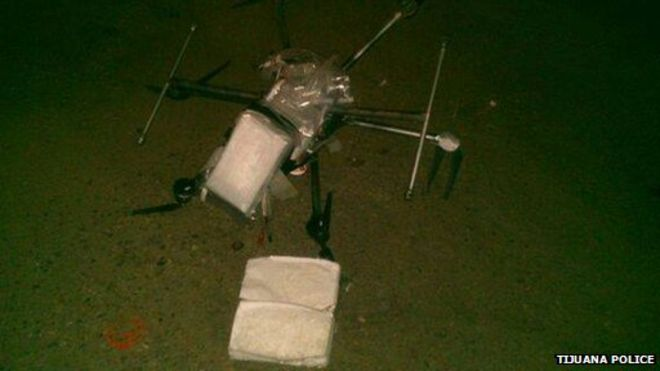
\includegraphics[scale=0.6]{pic/03_our-copter/drug.jpg}
  \end{figure}
  
\end{frame}



\begin{frame}
\frametitle{Controller, Modes}

  \begin{itemize}
    \item Stabilize    
    \item Waypoints   
	\item Acrobat
	\item Manual 
	\item 8 additional modes 
>>>>>>> origin/master
  \end{itemize}
  
\end{frame}


<<<<<<< HEAD
\begin{frame}
\frametitle{GPS navigation}

  %\begin{figure}
  %\includegraphics[scale=0.6, trim={5cm 8.5cm 5.5cm 8.5cm},clip]{pic/03_content/Serial_output.pdf}
  %\end{figure}
=======

\begin{frame}
\frametitle{Tool, Waypoint}

  \begin{figure}
  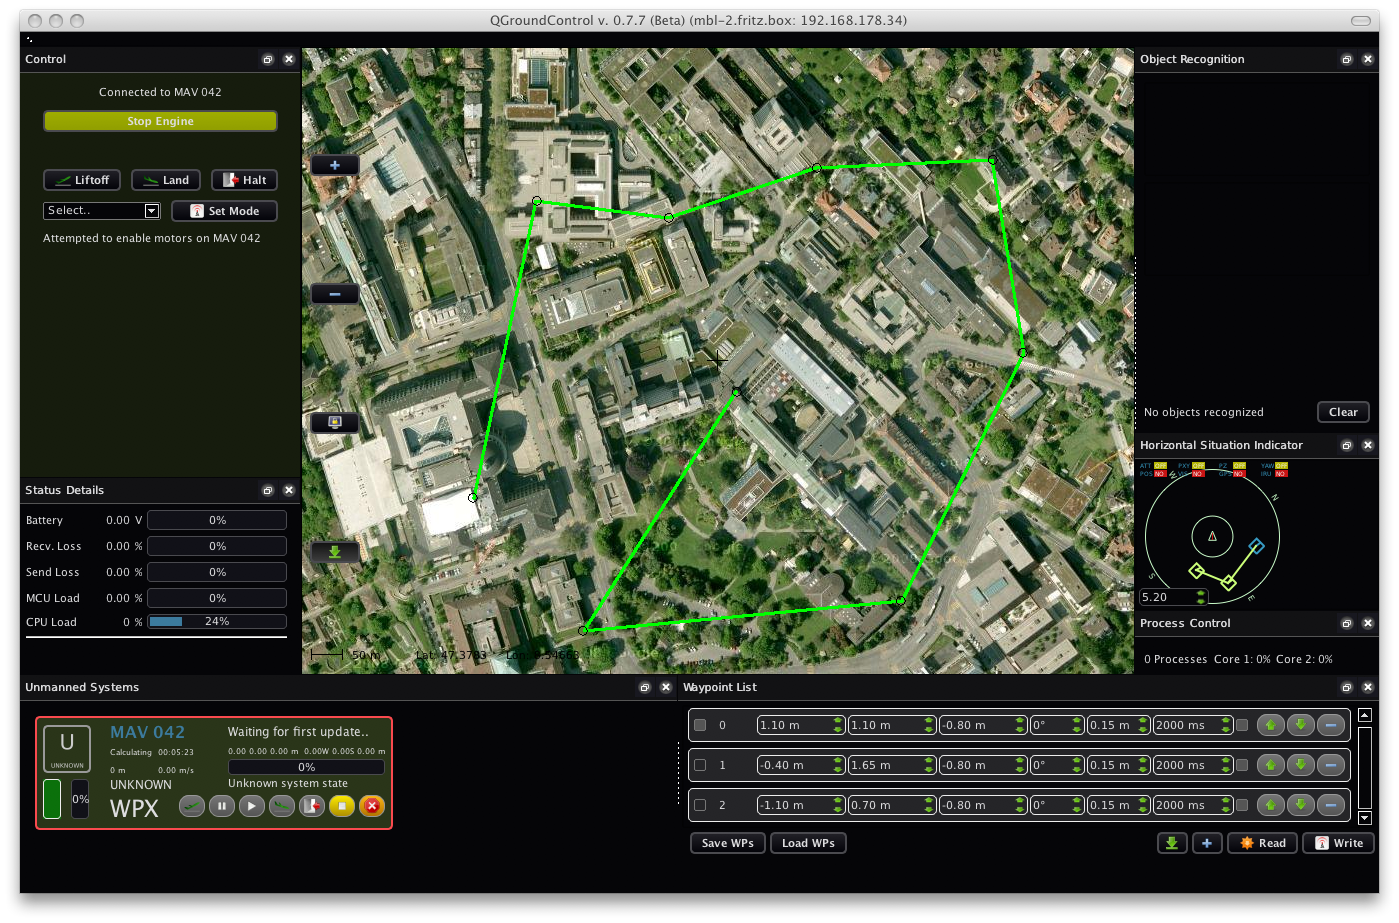
\includegraphics[scale=0.2]{pic/03_our-copter/qgroundcontrol.png}
  \end{figure}
>>>>>>> origin/master
  
\end{frame}



<<<<<<< HEAD

\begin{frame}
\frametitle{Stabilize}

  \begin{itemize}
    \item ....    
  \end{itemize}
=======
\begin{frame}
\frametitle{Gimbal}

  \begin{figure}
  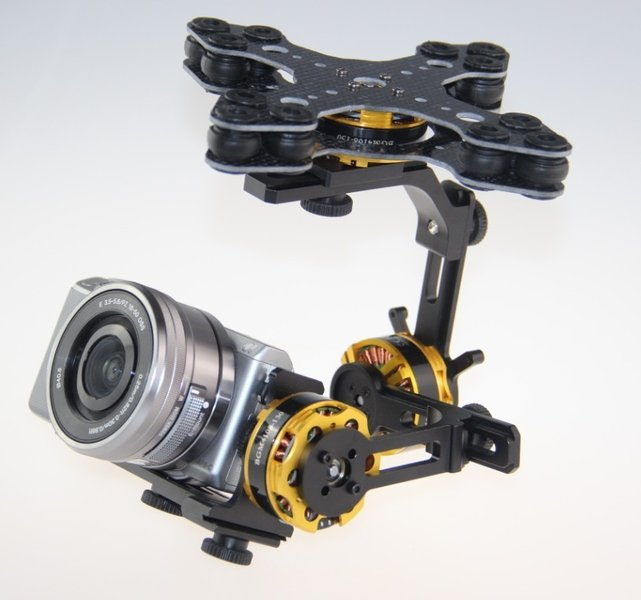
\includegraphics[scale=0.4]{pic/03_our-copter/gimbal.jpg}
  \end{figure}
>>>>>>> origin/master
  
\end{frame}



<<<<<<< HEAD

\begin{frame}
\frametitle{Accuracy}

  \begin{itemize}
    \item ....    
=======
\begin{frame}
\frametitle{First Person View}

  \begin{itemize}
    \item Transmitter    
    \item Receiver   
	\item Black \& white picture
	\item Noise 
>>>>>>> origin/master
  \end{itemize}
  
\end{frame}




<<<<<<< HEAD
=======



>>>>>>> origin/master
